\clearpage
\subsection{Software}

\begin{figure}[ht]
    \begin{center}
        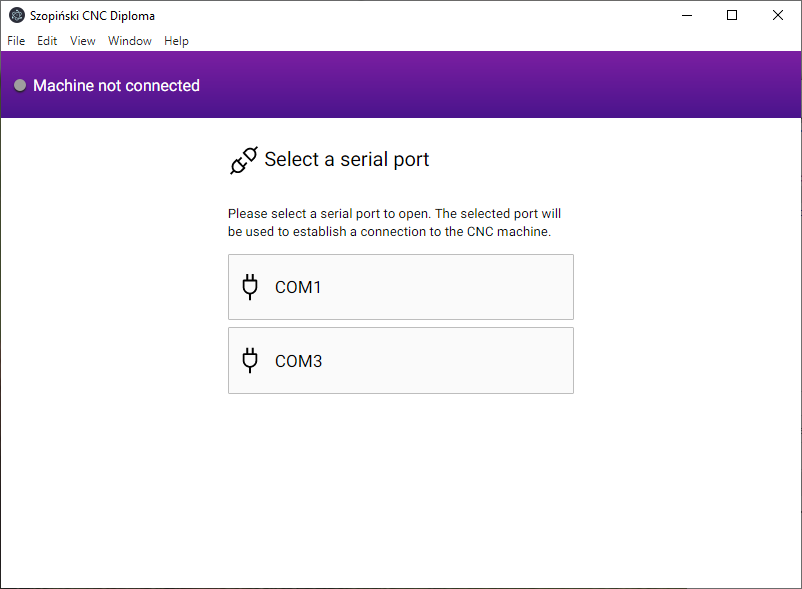
\includegraphics[width=0.75\linewidth]{serialselect}
        \caption{Serial port selection screen of the control software.}
        \label{serialselect}
    \end{center}
\end{figure}

The control software is implemented using Electron, a framework for writing
desktop applications using web technologies. This allows it to present an
elegant, modern user interface while retaining the ability to perform low-level
operations such as serial communication. It also makes it easy to achieve
cross-platform compatibility.

Electron applications are written in JavaScript. They consist of a main process,
which interacts with the operating system, and a renderer process, which
displays the user interface in a browser window and exchanges information with
the main process. This ensures security in case the renderer process becomes
compromised.

Web development practices favor the use of externally developed software to
solve commonly encountered problems. Such software is distributed in the form of
packages and installed by a package manager. Every project has a list of
dependencies which must be collected before it is run.

The following libraries and tools were used to create this application:

\begin{itemize}
    \item Yarn, a combined package manager and project manager. Used for
    managing dependencies and launching build utilities.
    \item Webpack, a module bundler. Needed to compile the project into a
    compact set of files suitable for consumption by Electron.
    \item React, a framework for building user interfaces. It introduces a
    system of components and a mechanism to coordinate the flow of information
    within the application.
    \item React Redux, a library for managing the global application state.
    Facilitates handling events which impact multiple unrelated parts of the
    user interface.
    \item React Router, a library to handle screen navigation.
    \item Node SerialPort, a JavaScript wrapper around the operating system's
    serial interface.
    \item Sass, a dialect of CSS which introduces a hierarchical structure.
    \item ESLint, a code analysis tool for detecting errors and enforcing code
    style.
\end{itemize}

Because the application does not fetch data from the Internet nor does it
execute code from the file system, the renderer process is allowed to interact
with the operating system directly. This simplifies program design by removing
the need to communicate with the main process. The main process is thus reduced
to boilerplate code which opens the browser window and loads an HTML document
containing the application.

\subsubsection{Global program state}

\begin{figure}[ht]
    \begin{center}
        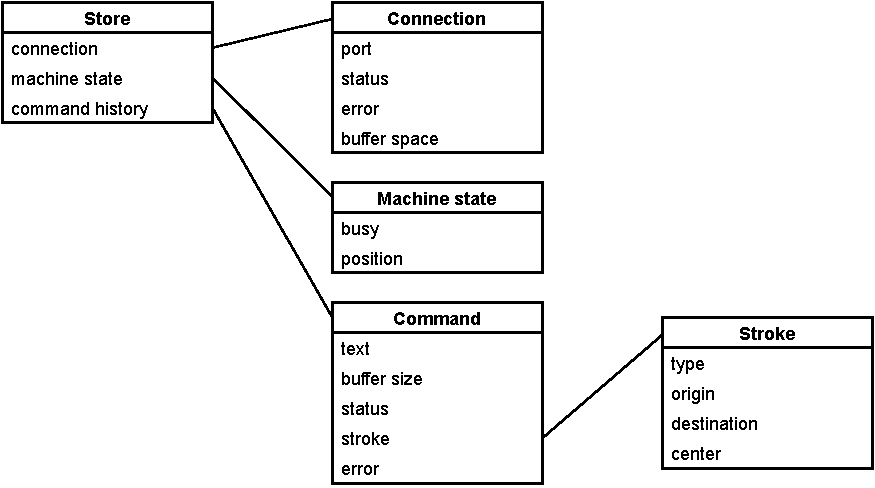
\includegraphics[width=0.75\linewidth]{globalstate}
        \caption{Structure of the store.}
        \label{store}
    \end{center}
\end{figure}

Main program functionality is centered around the global state object, which
by Redux terminology is referred to as the \textit{store}. Redux introduces the
following design principles \cite{redux}:
\begin{enumerate}
    \item The store may only be changed by dispatching \textit{actions}, which
    may be thought of as events. Actions are dispatched in response to user
    interaction or incoming or outgoing serial traffic. Actions are handled
    by \textit{reducer} functions, which dictate how they impact the store.
    \item Changes in the store may be \textit{subscribed to} by various
    components of the program. When subscribers detect that a relevant part
    of the store has changed, they may trigger appropriate behavior.
\end{enumerate}

The store is divided into three top-level objects (figure~\ref{store}):
connection state, machine state, and command history. Changes to the connection
state cause the program to establish or to close a serial connection. The
machine state object reflects feedback received from the device, and is observed
by the user interface. The command history object governs data transmission
to the device and allows the user to monitor the execution of commands.

\subsubsection{Serial communication}

\begin{figure}[ht]
    \begin{center}
        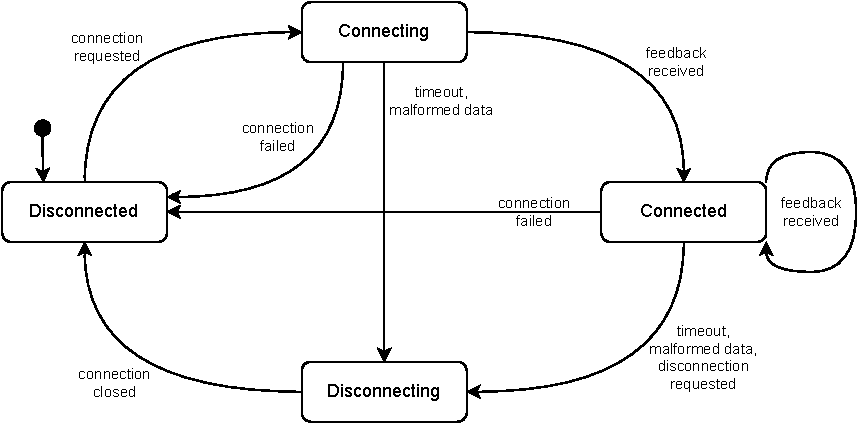
\includegraphics[width=0.75\linewidth]{serialstate}
        \caption{State transition of the serial connection.}
        \label{serialstate}
    \end{center}
\end{figure}

A global store subscriber is registered to handle serial communication. When the
user first launches the application, they are presented with a serial port
selection screen (figure~\ref{serialselect}). Choosing one of the options
changes the connection status to \texttt{connecting}. The subscriber detects
this change and attempts to establish a new serial connection.

The device sends three kinds of feedback. The software verifies that the
feedback is received within a certain time frame and that it isn't malformed.
Violating the serial protocol terminates the connection. Receiving valid
feedback marks the connection as established (see figure~\ref{serialstate}).

There are three kinds of feedback:

\begin{itemize}
    \item Position feedback, sent every quarter second. Receiving this packet
    updates the store's machine state and establishes the connection.
    \item ``Command started'' feedback, sent once a command has been executed
    but before its motion has finished. Contains an interpretation of the
    command by the machine's G-code parser. Receiving this packet updates
    the command history and triggers an attempt to send commands to the device
    (see next section).
    \item ``Command finished'' feedback, sent once the motion initiated by a
    command has finished or if there was no motion. Updates the command history.
\end{itemize}

\subsubsection{Command history and queue}
\label{sending}

\begin{figure}[ht]
    \begin{center}
        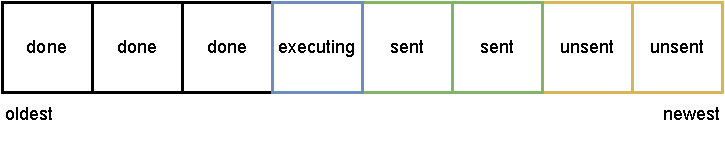
\includegraphics[width=0.6\linewidth]{commandhistory}
        \caption{Lifecycle of commands within the command history.}
        \label{commandhistory}
    \end{center}
\end{figure}

In order to maintain a logical connection between sent commands and received
feedback, the application maintains a global command history object to
coordinate the exchange of data between the software and the firmware
(see figure~\ref{commandhistory}).

A command begins its lifecycle when a \texttt{sendCommand} action is dispatched.
The new command, whose status is \texttt{unsent}, is placed at the end of the
command history. The serial communication subscriber observes the history and
attempts to send the command, provided there are no other sent commands.

The device's receive buffer is limited in size and cannot handle an overflow
condition. For this reason, the software keeps track of the amount of available
buffer space and delays the transmission of commands as necessary. If the
command's content, encoded as UTF-8, is within this limit, the command is sent.
Its status is set to \texttt{sent} and its size is subtracted from the
available buffer space.

Once sent, the command is read and executed by the machine. When feedback
arrives, the command is marked as \texttt{executing}, its interpretation and
error code are updated, and its size is added back to the buffer space.
This prompts an attempt to send more commands.

Finally, once the command has been executed, its status is set to \texttt{done}.
Executed commands are purged from the history when no longer relevant to the
user.

\subsubsection{Motion preview generation}

When the application is launched, the user is presented with a workflow
selection screen (figure~\ref{workflow}). They may choose from three different
workflows: batch execution, command prompt and bitmap tracing. The first two
screens are simple interfaces exposing the functionality described in
section~\ref{sending}.

In each screen, the user may view a list of executing commands and a preview
of the motion initiated by them (figures~\ref{batch} and~\ref{commandprompt}).
The preview is generated by translating motion interpretation objects
(received as feedback from the machine) into SVG tags embedded directly in the
HTML document.

\clearpage
\begin{figure}[ht]
    \begin{center}
        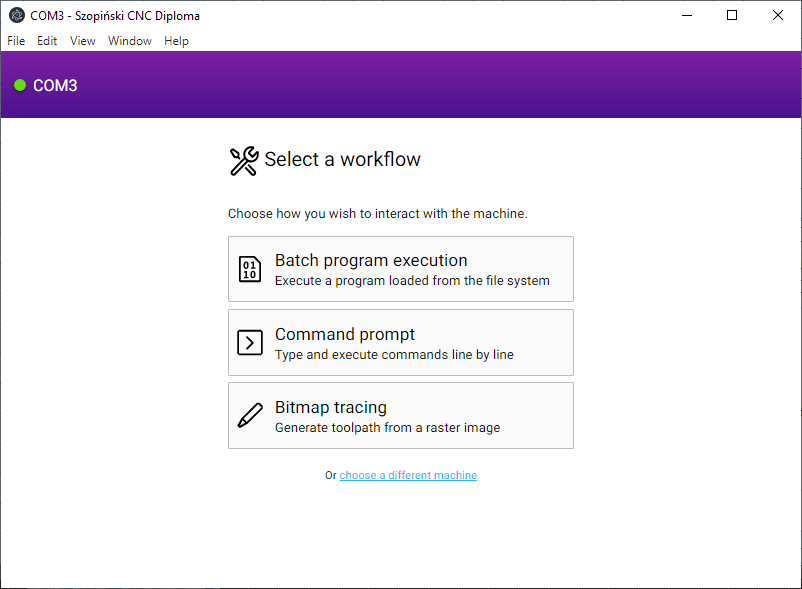
\includegraphics[width=0.8\linewidth]{workflowselect}
        \caption{Workflow selection screen.}
        \label{workflow}
    \end{center}
\end{figure}
\begin{figure}[ht!]
    \begin{center}
        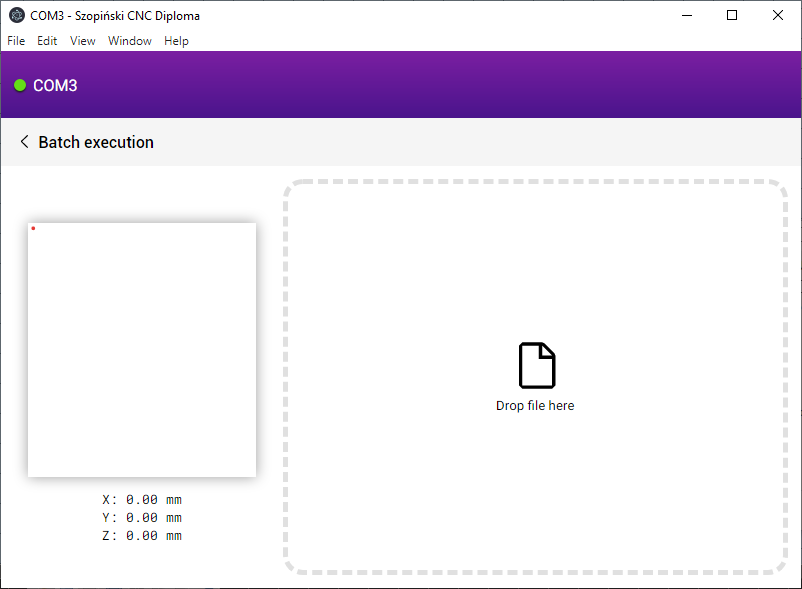
\includegraphics[width=0.8\linewidth]{batch}
        \caption{Batch execution screen, before dropping a file.}
    \end{center}
\end{figure}

\clearpage
\begin{figure}[ht]
    \begin{center}
        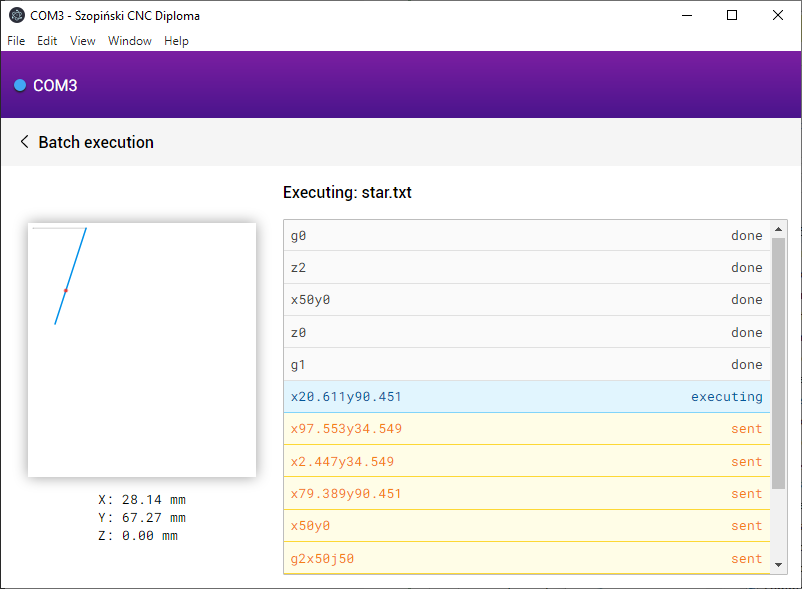
\includegraphics[width=0.8\linewidth]{batchexecuting}
        \caption{Batch execution screen, during execution.}
        \label{batch}
    \end{center}
\end{figure}
\begin{figure}[ht!]
    \begin{center}
        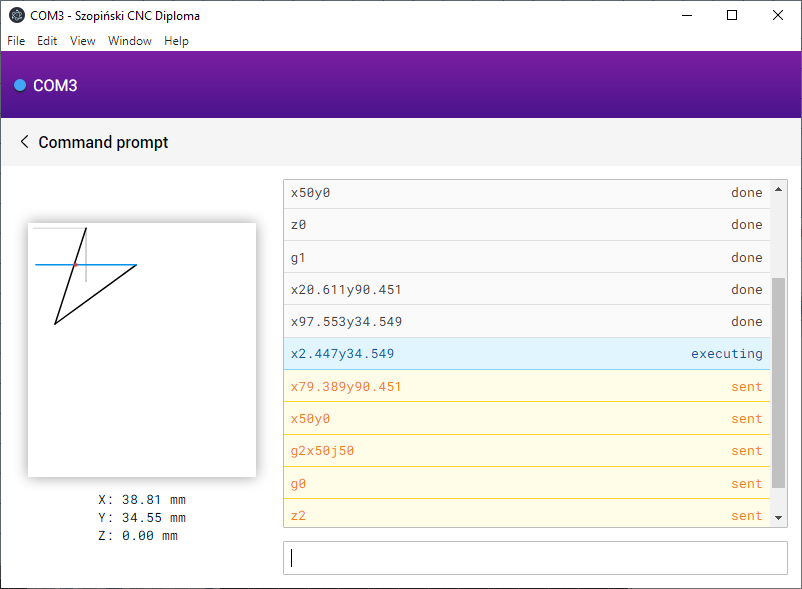
\includegraphics[width=0.8\linewidth]{commandprompt}
        \caption{Command prompt screen.}
        \label{commandprompt}
    \end{center}
\end{figure}

\clearpage
Translating linear motion is trivial. The SVG \texttt{line} element takes
arguments specifying the origin and the destination, which are given directly.
Rapid motion requires additional calculations for checking if it should be
split into two lines (as depicted in figure~\ref{rapid}). Circular motion,
however, takes significant effort to translate.

In SVG, there are two ways to describe arcs. Full arcs may be drawn using the
\texttt{circle} element, which takes a radius and a center point. Partial
arcs can only be drawn with the \texttt{path} element and its \texttt{A}
instruction. Because there are several paths through which two points may be
connected by an arc \cite{circles}, the \texttt{A} instruction takes many
arguments:

\begin{itemize}
    \item Implicit arc origin, set by the $M$ instruction
    \item $x$-axis radius and $y$-axis radius (equal for circles)
    \item $x$-axis rotation (irrelevant for circles)
    \item Large arc flag
    \item Sweep flag
    \item Arc end
\end{itemize}

The translation starts by calculating the radius:
\begin{equation*}
    R = \sqrt{(x_{dest} - x_{center})^2 + (y_{dest} - y_{center})^2}
\end{equation*}
If the origin and the destination are the same, a \texttt{circle} element is
rendered and the calculation ends.

\clearpage
\subsubsection{Bitmap tracing}
